\documentclass{beamer}

\usetheme{CambridgeUS}
\usepackage{graphicx}
\usepackage{caption}
\usepackage{subcaption}
\usepackage{listings}
\usepackage[style=authoryear]{biblatex}
\bibliography{hmm}

\begin{document}

\begin{frame}[t]
	\frametitle{A simple symbol recognition application}
	Features:
	\pause
	\begin{block}{Define}
		Define, organize and visualize a dataset of symbols defined with mouse movements.
	\end{block}
	\pause
	
	\begin{block}{Train}
		Train a HMM-based recognition engine on a symbol dataset.
	\end{block}
	\pause
	
	\begin{block}{Recognize}
		Recognize new symbols and view classification metrics.
	\end{block}
	\pause
	
	\begin{block}{}
		Default included symbols: \textbf{\emph{left arrow, right arrow, circle, square, infinity}}
	\end{block}
\end{frame}

\begin{frame}[t]
	\frametitle{A simple symbol recognition application - A View}
	
	\begin{figure}
  		\centering
		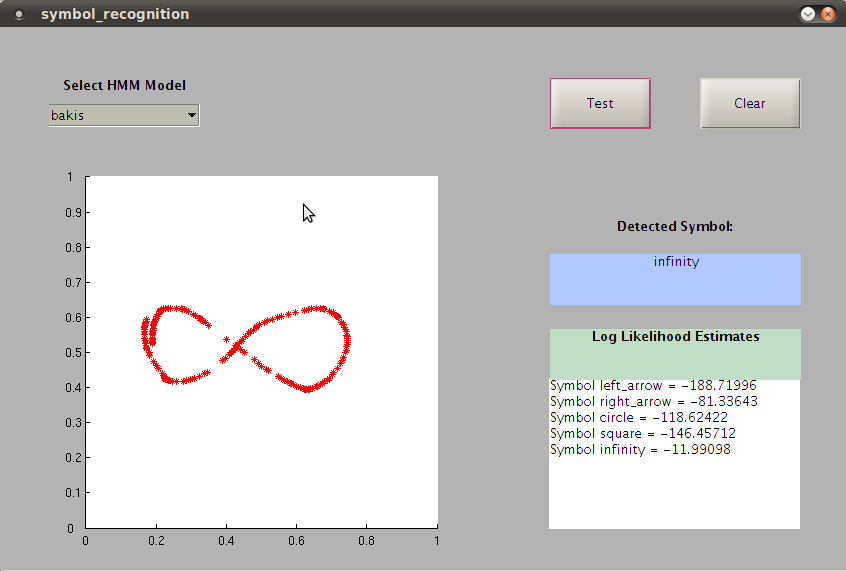
\includegraphics[height=0.70\textheight]{images/infinity.png}
		\caption{\tiny{A view of the symbol recognition application GUI}}
		\label{fig:baum-welch-alg}
  	\end{figure}	
\end{frame}

\begin{frame}[t]
	\frametitle{A simple symbol recognition application - Approach (I)}
	Adapted from \parencite{yang1994hidden}.
	\vspace*{1em}
	
	\only<1>{\centering 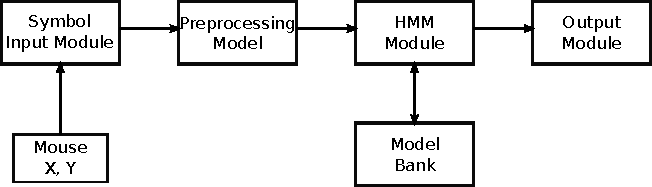
\includegraphics[width=0.85\textwidth]{images/symbol-app-architecture-1.pdf}}
	\only<2>{\centering 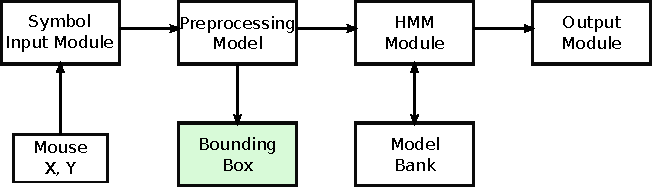
\includegraphics[width=0.85\textwidth]{images/symbol-app-architecture-2.pdf}}
	\only<3>{\centering 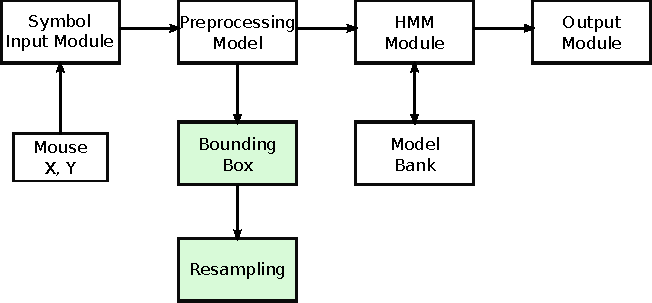
\includegraphics[width=0.85\textwidth]{images/symbol-app-architecture-3.pdf}}
	\only<4>{
		\centering 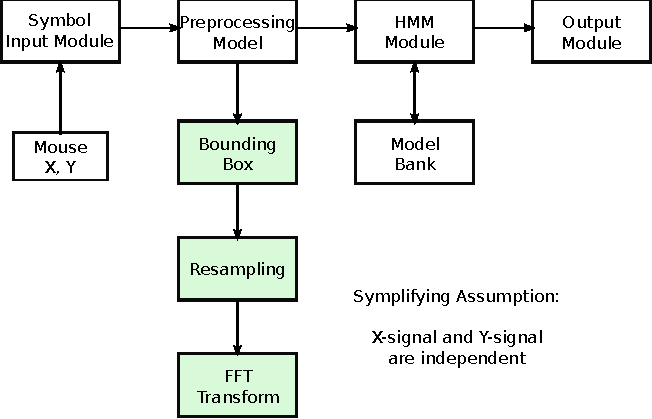
\includegraphics[width=0.85\textwidth]{images/symbol-app-architecture-4.pdf}	
	}
	
\end{frame}

\begin{frame}
	\frametitle{A simple symbol recognition application - Approach (II)}
	Adapted from \parencite{yang1994hidden}.
	
	\begin{block}{HMM Structure}
		$N$(number of states) = 8\\
		2 discrete observable variables per state - $coef_{FFT}(x)$, $coef_{FFT}(y)$\\
		$M$(number of values for each observable variable) = 256\\
		Transition model:\\
		\begin{itemize}
			\item Bakis
			\item Ergodic
		\end{itemize}
	\end{block}
	
\end{frame}

\begin{frame}[t]
	\frametitle{A simple symbol recognition application - Results}
	\scriptsize
	\begin{block}{Dataset size}
		\textbf{5} symbols: \textbf{\emph{left arrow, right arrow, circle, square, infinity}}\\
		\textbf{100} samples per symbol: \textbf{50} training, \textbf{10} validation, \textbf{40} testing
	\end{block}
	\normalsize
	
	\begin{columns}[T]
		\column{0.5\textwidth}
		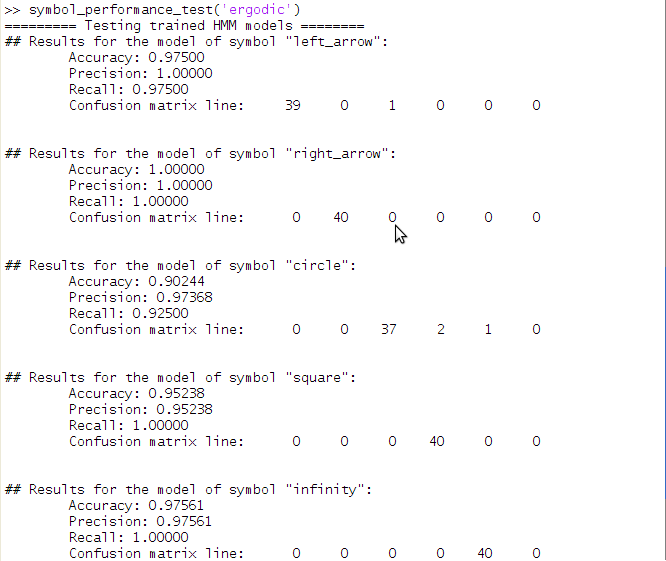
\includegraphics[width=\textwidth]{images/results-ergodic.png}
		\column{0.5\textwidth}
		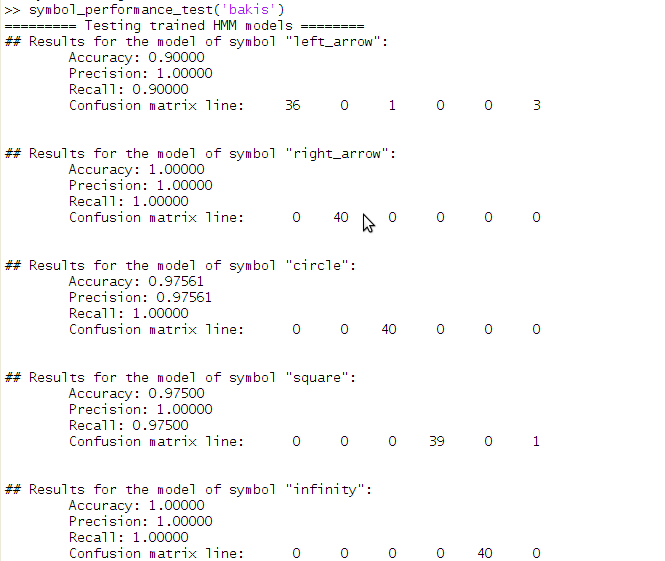
\includegraphics[width=\textwidth]{images/results-bakis.png}
	\end{columns}
\end{frame}

\end{document}